% 完成时间 2018/12/3 
\documentclass[a4paper, 12pt, oneside]{article}
\usepackage{resume}

\begin{document}
\newcommand\myworries[1]{\textcolor{red}{#1}}
\pagestyle{empty}
    % \noindent\begin{minipage}[t]{0.6\linewidth}
    \begin{tcolorbox}[colback=red!58!white,colframe=red!75!black]
        \Large \textit{张亚栋} \hfill\textsubscript{\raisebox{0pt}[0pt][0pt]{\large\faHeartO\raisebox{0.3ex}{\fontsize{12pt}{12pt}\faHeartO}%
    %\raisebox{0.7ex}{\faHeartO\faHeartO}%
    %\raisebox{1.2ex}{\faHeartO}%
    \raisebox{2.2ex}{\fontsize{11pt}{11pt}\faHeartO}%
    \raisebox{4.5ex}{\fontsize{10pt}{10pt}\faHeartO}
    \LaTeX
}}
    \end{tcolorbox}
    \begin{minipage}[t]{0.6\linewidth}
    \noindent
    \textcolor{red}{\faGraduationCap} 华东师范大学·学前教育学~\emph{本科}\\
    \textcolor{black}{\faCalendar}~ \emph{2015.09 - 2019.06}\\
    \textcolor{blue}{\faMars}~ \emph{1997-09-19}\\
    \textcolor{yellow}{\faMapMarker}~ 上海市普陀区中山北路3663号\\
    \textcolor{cyan}{\faEnvelope}~ $\mathsf{10154508169@stu.ecnu.edu.cn}$ \\ 
    \textcolor{black}{\fontsize{18pt}{18pt}\faMobile}~ (+86)\textbf{\emph{152-0170-6690}}
    % \faGithubAlt~\href{https://github.com/Tom007Cheung}{Github$-$Tom007Cheung}
    \end{minipage}
    \begin{minipage}[t]{0.1\linewidth}
    \begin{center}
        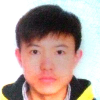
\includegraphics{photo.png}
    \end{center}
    \end{minipage}
    \begin{shadequote}{}
    \par
        \emph{A Renaissance person, also a Rookie !}
    \par
    \end{shadequote}
    \begin{tcolorbox}[enhanced,attach boxed title to top center={yshift=-3mm,yshifttext=-1mm},
  colback=yellow!10!white,colframe=yellow,colbacktitle=red!80!black,
  title={在校经历},fonttitle=\bfseries, fontupper=\CTEXindent,
  boxed title style={size=small,colframe=red!50!black}]
      \begin{tcolorbox}[colback=yellow!58!white,colframe=yellow!75!black]
    \begin{description}
        \item [2015.11] ~~汉字应用水平测试~~~~~~\emph{二级}
    \end{description}
\end{tcolorbox}
      \begin{tcolorbox}[colback=yellow!58!red,colframe=orange!75!black]
    \begin{description}
        \item [2016.04] ~~BAP 认证\emph{(海峡赛)} \emph{初级}
        \item [2016.06] ~~大学生英语四级考试 ~~\emph{530}
    \end{description}
\end{tcolorbox}
      \begin{tcolorbox}[colback=red!58!yellow,colframe=red!80!black]
    \begin{description}
        \item [2017.03] ~~普通话水平测试~~~~~~~~~~~\emph{二级乙等}
        \item [2017.06] ~~编程学习
    \end{description}
\end{tcolorbox}
      \begin{tcolorbox}[colback=red!58!white,colframe=red!75!black]
    \begin{description}
        \item [2018.02] ~~\href{https://github.com/Tom007Cheung/resume}{\LaTeX 排版}
    \end{description}
\end{tcolorbox}
    \end{tcolorbox}
    
\end{document}